%\chapter{Main Results}
\chapter{提案手法}


本研究では「2層の畳み込みニューラルネットワークに構造特徴を追加したモデル」にattentionメカニズムを適応したモデルを提案する。モデルの概要は以下の通りである。
\begin{figure}[htbp]
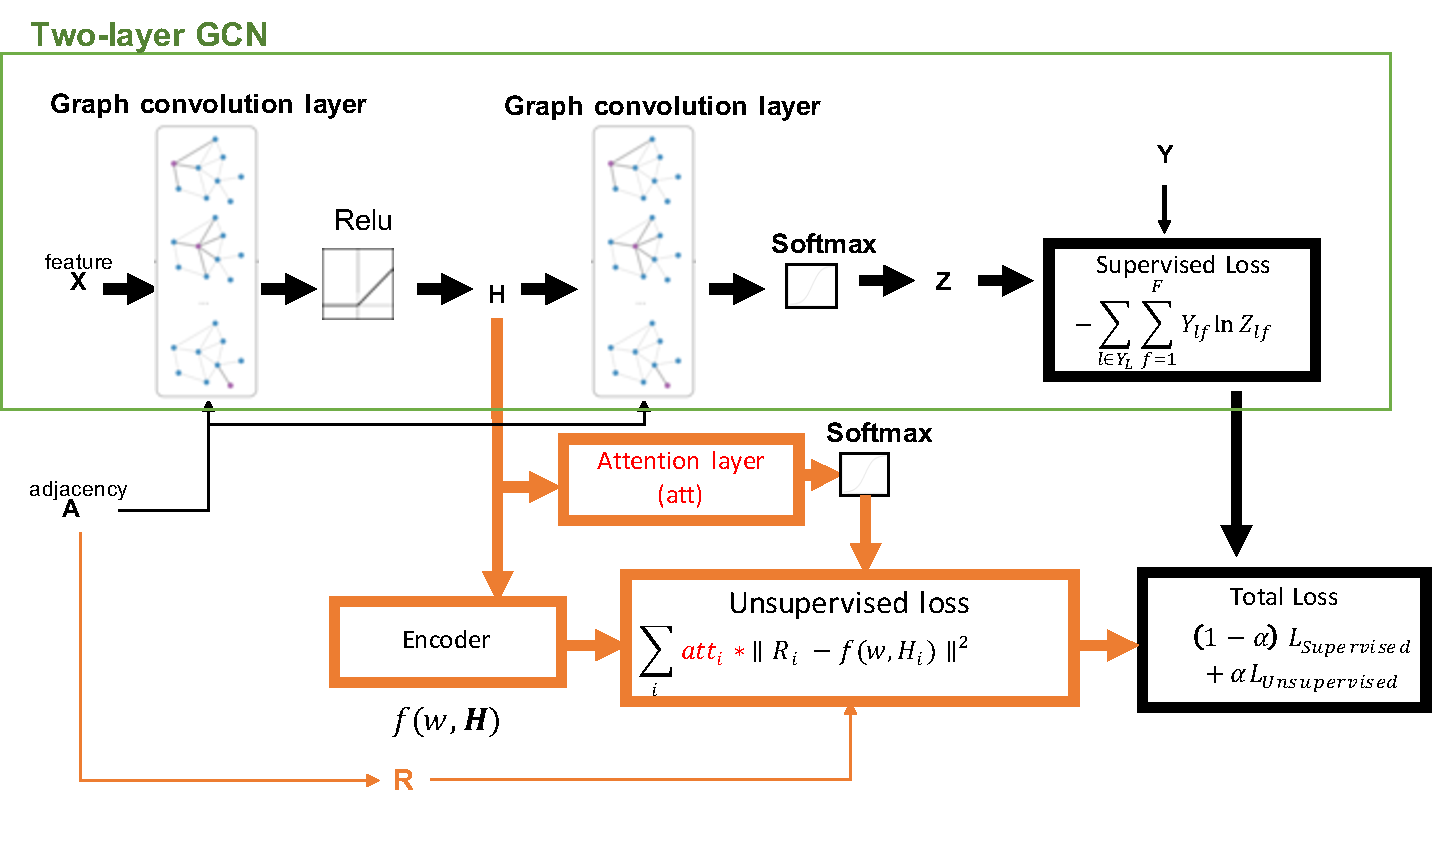
\includegraphics[width=1.0\hsize]{figures/proposed2.pdf}
\caption{提案手法(2層GCNを用いたモデル)}
\label{fig:architecture}
\end{figure}
\\
\\
\section{提案手法}
提案手法の図は図3.1に示す。図の上側にある緑枠で囲まれた部分はGCNの元論文の実装と等しい畳み込みネットワークである。図の下側にあるネットワークは構造特徴を用いて損失関数を出力する層になっている。提案手法においては本来のGCNで求める教師あり学習と構造特徴にattentionメカニズムを組み込んで求める教師なし学習、これら二つの目的関数を最適化するような目的関数を求めるものである。具体的にはトレードオフパラメータ$\alpha $を用い以下のような目的関数を実装することにより実現している。
\begin{equation}
L = (1-\alpha) L_{supervised} + \alpha L_{unsupervised}
\end{equation}
ここで、$L_{supervised}$は教師あり学習の損失関数、$L_{unsupervised}$は教師なし学習の損失関数である。
教師あり学習の損失関数は教師データのラベルのみを使い学習され、教師なし学習の損失関数は全てのノードにおいて学習される。また、およその流れは以下の図のようになっている。
\begin{figure}[htbp]
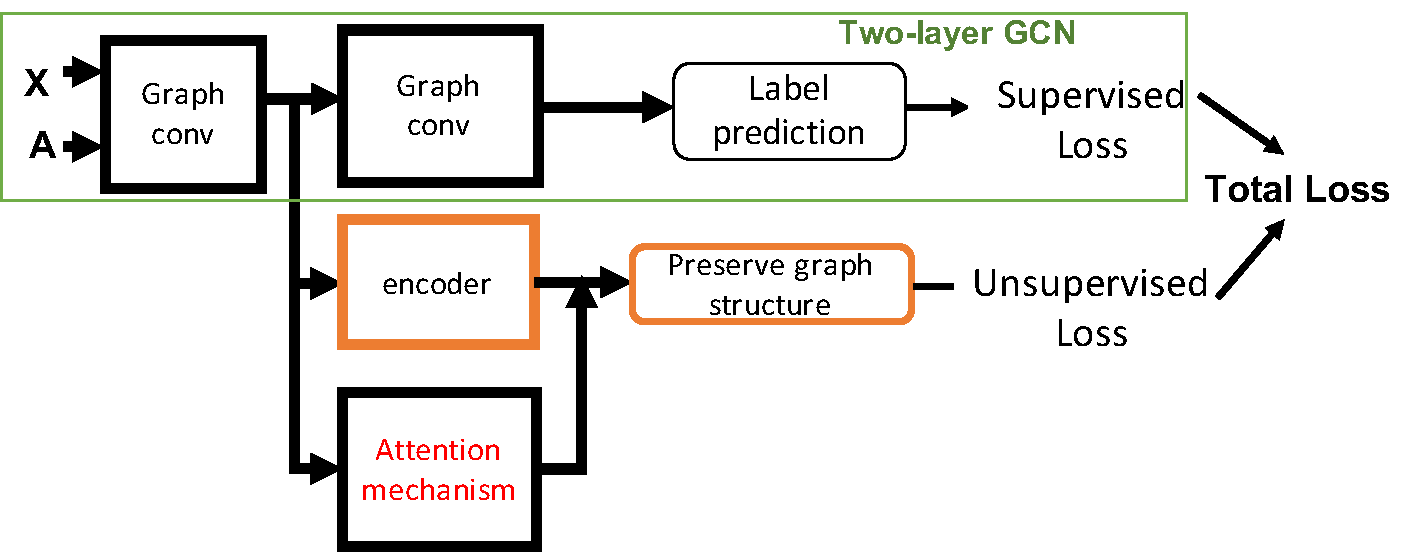
\includegraphics[width=1.0\hsize]{figures/proposed.pdf}
\caption{提案手法のおよその流れ}
\label{fig:flow}
\end{figure}
\section{教師あり学習における損失関数}
教師あり学習においては,\cite{gcn}でのラベル予測学習で用いられる損失関数と同様の損失関数を用いる。入力には隣接行列Aと特徴行列Xを使用し、ニューラルネットワークにおける順伝搬によって演算が行われる。ここで、特徴行列Xは、それぞれのノードが個別に持っているそのノードの特徴を表す行列である。ネットワーク$i$層における出力は以下のようになる。
\begin{equation}
Z^{(i)} = \sigma(D^{-1/2}\tilde{A}D^{-1/2}Z^{(i-1)}W^{(i)})
\end{equation}
ここで,$\tilde{A}=A+I_{n}$,$I_{n}\in R^{n \times n}$は単位行列であり、$\tilde{D_{i,j}}$は、
\begin{equation}
\tilde{D_{i,j}} = \begin{cases}
    \sum_j \tilde{A_{i,j}} & (i==j) \\
    0 & (otherwise)
  \end{cases}
\end{equation}
である。\\

ネットワークの入力ベクトル$Z^{(0)}$を特徴ベクトルX,$W^{(i)}$をネットワーク中の$i$層における重み行列であり,$\sigma(.)$はReLU関数やシグモイド関数などの活性化関数とすると、畳み込み層が2層のニューラルネットワークを用いて,活性化関数を1層目にRelu、2層目にsoftmax関数を用いたとすると、出力は以下のように表される。
\begin{equation}
Z = f(X, A) = {\rm softmax}(\hat{A}{\rm ReLU}(\hat{A} XW^{(0)})W^{(1)})
\end{equation}





ここで、$ \hat{A} = \tilde{D}^{-1/2} \tilde{A} \tilde{D}^{-1/2} $と置く。$W^{(0)} \in \mathcal{R}^{C\times H}$は入力層から隠れ層へ変換するための重み行列であり、$W^{(1)} \in \mathcal{R}^{H\times F}$は,隠れ層から出力層へ変換するための重み行列である。変数C,H,Fはそれぞれ入力層、隠れ層、出力層のサイズを表すパラメータであり、Cは特徴量の次元数、Hはハイパーパラメータ、Fはノードのラベルの種類数によって定まる。損失関数は、ラベル付きノードにおいてのクロスエントロピーにより求められる。教師あり学習における損失関数は以下のようになる。
\begin{equation}
L_{supervised} = - \sum_{l \in Y_{l}} \sum_{f=1}^{F} Y_{lf} lnZ_{lf}
\end{equation}
ここで$Y_{l}$はラベル付けされたノードの場合1、それ以外で0で表される。


\section{教師なし学習における損失関数}
まず、構造特徴を保持するための学習についての詳細を説明する.

\subsection{構造特徴行列の計算}
構造特徴は、入力行列である隣接行列により、各ノードごとの構造特徴をそれぞれ計算される。提案手法で用いる構造特徴はノードごとに計算される中心性である、媒介中心性、近接中心性、次数中心性、固有ベクトル中心性、pagerankなどである。それぞれのノードごとの特徴量を全ての構造特徴において結合したものを構造特徴行列$ R\in R^{N\times S}$とする。Nはノード数、Sは用いる構造特徴の総数である。この構造特徴は使うデータセット によって一意に定まるため、一度計算したら再度計算する必要性はないため、モデル全体の計算量に対する影響はとても低い。

\subsection{特徴ベクトルの計算}

提案手法においては、2層のグラフ畳み込みネットワークを用いる。1層目の畳込み層の関数を$GCN_1$、2層目の畳込み層の関数を$GCN_2$とすると、グラフ畳み込みネットワークにおける順伝播は以下の式で表せる。\\
\begin{eqnarray}
H_{hid} = GCN_1(X,A)\\
H_{out}=GCN_2(H_{hid} , A)
\end{eqnarray}
構造特徴保持のための学習を$H_{hid}$からそれぞれのノードにおける特徴ベクトル$\hat{R}$を計算する層を導入する。2層のグラフ畳み込みネットワークを用いる場合は、1層目の畳み込み層における出力から派生させて特徴ベクトルを計算する。それぞれのノードにおける重みパラメータ{\bf $\omega$}を用いることで特徴ベクトル$\hat{R} \in R^{N\times S}$は以下のように計算できる。
\begin{equation}
\hat{R} = f(w, H_{hid})
\end{equation}

\subsection{attentionの計算}
構造特徴の保持を行うために、出力された特徴ベクトルがグラフそのものから計算された構造特徴との差異ができるだけ小さくなるように学習を行う。ここで、ノードごとに構造特徴の中で重要な構造特徴とそうでない構造特徴があるものに注目し、ノードごとに構造特徴にattentionメカニズムを組み込む。求める教師なし損失関数は、グラフから計算した構造特徴とグラフ畳み込みネットワークの1層から出力された特徴ベクトルの二乗誤差にノードごとの構造特徴においてattentionをかけたものとなる。
\begin{equation}
L_{unsupervised} = \sum_{i=1}^{N} att_i * ||R_{i} - \hat{R_{i}}||^{2}
\end{equation}
ここで、$att_i \in R^{S}$はノードiにおけるそれぞれの構造特徴にかかるattentionである。
